\documentclass[letterpaper,inpress,dvipsnames]{jdsart}

\setcounter{page}{1}
\pubmonth{July}
\pubyear{2022}
\volume{xx}
\issue{xx}
\doi{0000}


\usepackage[utf8]{inputenc}
\providecommand{\tightlist}{%
  \setlength{\itemsep}{0pt}\setlength{\parskip}{0pt}}

\usepackage{subfig}

\usepackage{amsfonts,amsmath,amssymb,amsthm} 
\usepackage{threeparttable}
\usepackage{cleveref}
\usepackage{booktabs} 
\usepackage{lipsum} 
\PassOptionsToPackage{dvipsnames}{xcolor} 
\newcommand{\svp}[1]{{\textcolor{ForestGreen}{#1}}} 
\newcommand{\tw}[1]{{\textcolor{Red}{#1}}}

\begin{document}
\begin{frontmatter}

\title{Evaluating Perceptual Judgements on 3D Printed Bar Charts}
\runtitle{Perceptual Judgements on 3D Printed Bar Charts}

\author[1]{
  \inits{T.}
  \fnms{Tyler}
  \snm{Wiederich}  \thanksref{1}  \ead{twiederich2@huskers.unl.edu}}
\author[1]{
  \inits{S.}
  \fnms{Susan}
  \snm{VanderPlas}  \ead{susan.vanderplas@unl.edu}}

\thankstext[type=corresp,id=1]{Tyler Wiederich}
\address[1]{Department of Statistics, 
  \institution{University of Nebraska-Lincoln}, \cny{United States of America}}

\begin{abstract}
Graphical design principles typically recommend minimizing the dimensionality of a visualization - for instance, using only 2 dimensions for bar charts rather than providing a 3D rendering, because this extra complexity may result in a decrease in accuracy. This advice has been oft repeated, but the underlying experimental evidence is focused on fixed 2D projections of 3D charts. In this paper, we describe an experiment which attempts to establish whether the decrease in accuracy extends to 3D virtual renderings and 3D printed charts. We replicate the grouped bar chart comparisons in the 1984 Cleveland \& McGill study, assessing the accuracy of numerical estimates using different types of 3D and 2D renderings.
\end{abstract}

\begin{keywords}
\kwd{graphics}\kwd{3D bar charts}\kwd{3D printing}.
\end{keywords}

\end{frontmatter}

\hypertarget{introduction}{%
\section{Introduction}\label{introduction}}

Good communication requires both that the information be transmitted correctly and that the intended recipient be able to decode and understand the transmitted information accurately. In order to communicate effectively, we must use graphical forms that accurately convey information relevant to the task in question. In many cases, this means we must understand how accurately people can read quantitative information off of charts. While accuracy is not the only quantity of interest in graphical investigations \citep{hullmanPursuitErrorSurvey2019}, it is an important factor in assessing the utility of many different data graphics.

The accuracy of graphical forms has been studied for almost a century \citep{vonhuhnFurtherStudiesGraphic1927, eellsRelativeMeritsCircles1926, croxtonGraphicComparisonsBars1932, croxtonBarChartsCircle1927}, as new ways of representing information evolve, we must revisit old studies to determine whether these representations have the same limitations as previous versions. This is particularly true in areas like graphics which are affected by the immense technological innovation in hardware and software which has taken place since the early 1990s.

\hypertarget{elementary-graphical-tasks}{%
\subsection{Elementary Graphical Tasks}\label{elementary-graphical-tasks}}

\citet{clevelandGraphical1984} established the comparative accuracy of different ``elementary perceptual tasks'' (EPTs).
Elementary Perceptual Tasks, according to these experiments, include assessing graphical elements such as position along a common scale, length, angle, and volume, and estimating the corresponding numerical value of these representations.
The study relied entirely on estimation accuracy, which may not always be relevant when extracting information from graphs. For example, estimation is less relevant when ordering values by size.
As a result of the Cleveland and McGill \citeyearpar{clevelandGraphical1984} study, it is possible to assemble an ordering of perceptual accuracy for the elements of length, position, and angle.
\citet{heerCrowdsourcingGraphicalPerception2010b} replicated some parts of \citet{clevelandGraphical1984} in an online setting using Mechanical Turk, largely validating the results of the original study while demonstrating the utility of the Mechanical Turk platform for graphical testing.

The first experiment in \citet{clevelandGraphical1984} (the position-length experiment), used five types of bar charts: two types of grouped bar charts and three types of stacked bar charts.
Each chart had two bars marked for comparison; participants were asked to determine which bar was smaller and give the perceived ratio of the smaller bar to the larger bar. \Cref{fig:bar-types} shows the two types of grouped bar charts.
We are primarily interested in the grouped bar charts (in part because 3D printing is not yet inexpensive enough to make moderate-scale stacked bar chart experiments viable), which consisted of two comparison bars which were either adjacent or in separate groups.
These grouped bar charts will be referenced as adjacent and separated graph types in this paper, respectively.

\begin{figure}
\includegraphics[width=.49\linewidth]{jds_files/figure-latex/bar-types-1} \includegraphics[width=.49\linewidth]{jds_files/figure-latex/bar-types-2} \caption{\citet{clevelandGraphical1984} used two different types of grouped bar charts: comparisons between adjacent bars, and comparisons between separated bars. It is widely acknowledged that comparisons between separated bars (Type 3 comparisons, in Cleveland \& McGill's terminology) are more difficult and error-prone.}\label{fig:bar-types}
\end{figure}

\hypertarget{d-graphical-perception}{%
\subsection{3D Graphical Perception}\label{d-graphical-perception}}

Chart perception is often affected by the visual system's implicit assumption that visual stimuli are three-dimensional; after all, most of the visual input we process does come from a three-dimensional world, but charts are artificial and largely exist in two dimensions.
This occasionally causes problems: the line-width illusion\citep{vanderplasSignsSineIllusion2015, daySineIllusion1991, hofmannCommonAnglePlots2013}, for instance, has been attributed to implicit 3D perception of 2D stimuli and can affect perception of error bands, candlestick plots, and Sankey diagrams (a simplified example is shown in \citet{fig:sine-illusion}).
While this illusion is problematic in 2D, when the depth cues are actually present in a three-dimensional situation, the same perceptual heuristics contribute to accurate size perception. Thus, there is reason to think that perceptual accuracy may be dependent on the realism of the stimuli.

\begin{figure}
\subfloat[Sine Illusion\label{fig:sine-illusion-1}]{\includegraphics[width=0.33\linewidth]{jds_files/figure-latex/sine-illusion-1} }\subfloat[3D surface with similar features\label{fig:sine-illusion-2}]{\includegraphics[width=0.33\linewidth]{jds_files/figure-latex/sine-illusion-2} }\subfloat[Perceived vs. actual length\label{fig:sine-illusion-3}]{\includegraphics[width=0.33\linewidth]{jds_files/figure-latex/sine-illusion-3} }\caption{An illustration of the sine illusion\citep{vanderplasSignsSineIllusion2015}, also known as the line-width illusion. All vertical lines are the same length, but the lines in the middle of the curve appear to be much shorter. The illusion results when implicit perceptual corrections useful for perceiving the size of objects with depth are applied to 2D stimuli with no actual depth. As 3D heuristics occasionally cause inaccurate communication when applied to 2D objects, it is reasonable to think that there might be some situations where charts making use of a realistic third dimension might be perceived more accurately than their 2D equivalents.}\label{fig:sine-illusion}
\end{figure}

The use of 3D graphics have been explored in multiple studies.
\citet{fisher_data_1997} explored user preference for 2D or 3D charts and found that subjects tended to prefer simpler 2D graphs when tasked with extracting information.
\citet{barfield_effects_1989} compared 2D and 3D graphs presented on paper and on computers, showing that the accuracy of subject answers depended on their skill level: novice subjects were more accurate with 2D paper graphs, while experienced managers were more accurate with 3D computer graphs.
For both experience levels, participants were more confident in their answers when using 2D graphs.
There are instances where 2D graphs perform better than 3D graphs, but there are times where 3D graphs may provide a more natural way to encode information, at least in theory. For instance, when X and Y are used to represent spatial dimensions, it may be preferable to use a 3D chart to convey numerical information instead of using color, which is perceived much less accurately.
\citet{brath_3d_2014} highlights the intrinsic attributes of 3D graphs and the benefits when used appropriately with other 3D elements such as lighting and correct portrayal of data attributes.

There is thus good reason to be wary of the use of three dimensions where only two are necessary to convey data \citep{vanderplasTestingStatisticalCharts2020, wilkeDonGo3D2020, morganwallIntroducing3DGgplots20191006}.
However, the situation is different now than it was in 1984 when Cleveland \& McGill published their seminal work; it has even changed since Heer's replication study \citeyearpar{heerCrowdsourcingGraphicalPerception2010b} in 2010.\\
Digital graphics have developed quickly, along with the hardware necessary to support these software developments.
As a result, we have much more natural rendering of 3D objects virtually, and we can also print graphics in three dimensions, moving artificial charts into a more natural, physical setting.
As a result, it is reasonable to reconsider the use of 3D charts, not only because of new technological developments, but also because these charts provide the opportunity to make data graphics accessible to those with limited or absent vision \citep{fleetHowTactileGraphics2023}.

In this paper, we discuss a study designed to examine Cleveland \& McGill's experiments on grouped bar charts using modern graphics in two and three dimensions. This study lays the groundwork for additional empirical studies on the use of 3D graphics, rendered and 3D printed, for visualizing complex data. In order to explore perception of fully 3D graphics, it is prudent to start with the simplest possible 3D graphic: one in which the third dimension is not necessary, so that we can easily compare to two-dimensional representations without loss of information.
In the next section we provide details about design and execution of our experiment, including the process of replicating stimuli from \citet{clevelandGraphics1984} in order to create 2D, 3D projected, 3D rendered, and 3D printed bar graphs. The next section presents the results, and we conclude the paper by discussing this experiment in the context of existing work on the perception of 2D and 3D graphical elements.

\hypertarget{methods}{%
\section{Methods}\label{methods}}

Our study is designed to replicate and expand upon the position-length experiment from Cleveland \& McGill as closely as possible, with the hope of being able to integrate this study with previously reported results in a consistent manner.
In this section, we discuss the replication process and the design of our version of this experiment.

\hypertarget{replicating-cleveland-and-mcgill}{%
\subsection{Replicating Cleveland and McGill}\label{replicating-cleveland-and-mcgill}}

The first step of replicating the position-length experiment was to determine the heights of the bars that participants use for comparisons.
These values for the bar heights are linear on a log scale and are given by

\[s_i=10\cdot 10^{(i-1)/12}, \qquad i=1,...,10\]

Each graph presents two bars from the values given above where the participants are asked to judge the ratio of the smaller bar to the larger bar. The ratio of bars used by Cleveland and McGill were 17.8, 26.1, 38.3, 46.4 (twice), 56.2, 68.1 (twice), and 82.5 (twice).
The exact numeric comparisons were not disclosed, but the comparison values used in our study were subjected to the constraints of having the same ratio values and that no value was used more than twice. {\textcolor{ForestGreen}{Can we show the comparison values in a table?}}

{\textcolor{ForestGreen}{In each graph, there are two sets of five bars each, and two of the bars are marked for identification with a circle and triangle}}, {\textcolor{ForestGreen}{as in \Cref{fig:bar-types}.}}
Cleveland and McGill did not specify the random process for the heights of the eight other bars, so we used a scaled Beta distribution with parameters that limit excessive noise around the bars used for comparisons.{\textcolor{ForestGreen}{What does excessive noise mean??}}
Code to reproduce the data generation process, data underlying the plots used in this study, the rendered plots and STL files, anonymized user data, and analysis code can found be at \url{https://github.com/TWiedRW/2023-JDS-3dcharts}.

\hypertarget{stimuli-construction}{%
\subsection{Stimuli Construction}\label{stimuli-construction}}

The graphs share a common layout across all formats, where two groupings of five bars are identified by ``A'' and ``B'', respectively, and circles and triangles are used to identify the bars participants should compare. Example graphs are shown in
\Cref{fig:plotTypes}.
There are some graphical elements that cannot be easily portrayed via 3D printing. For this reason, all graph types do not have axes, grid lines, or floating titles.

\begin{figure}
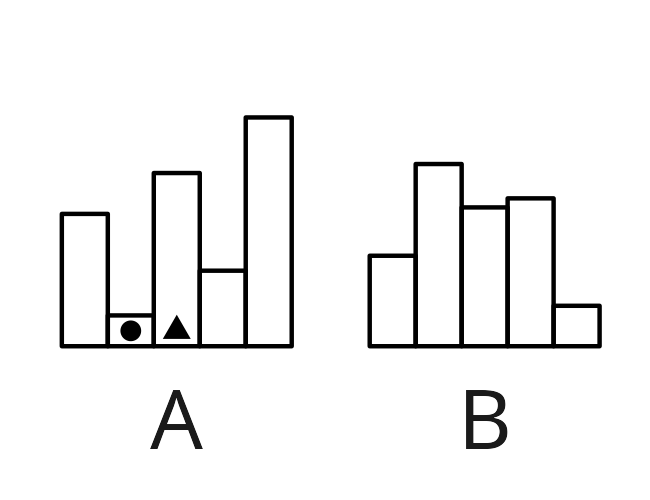
\includegraphics[width=0.3\linewidth]{_images/Type1-Rep01} 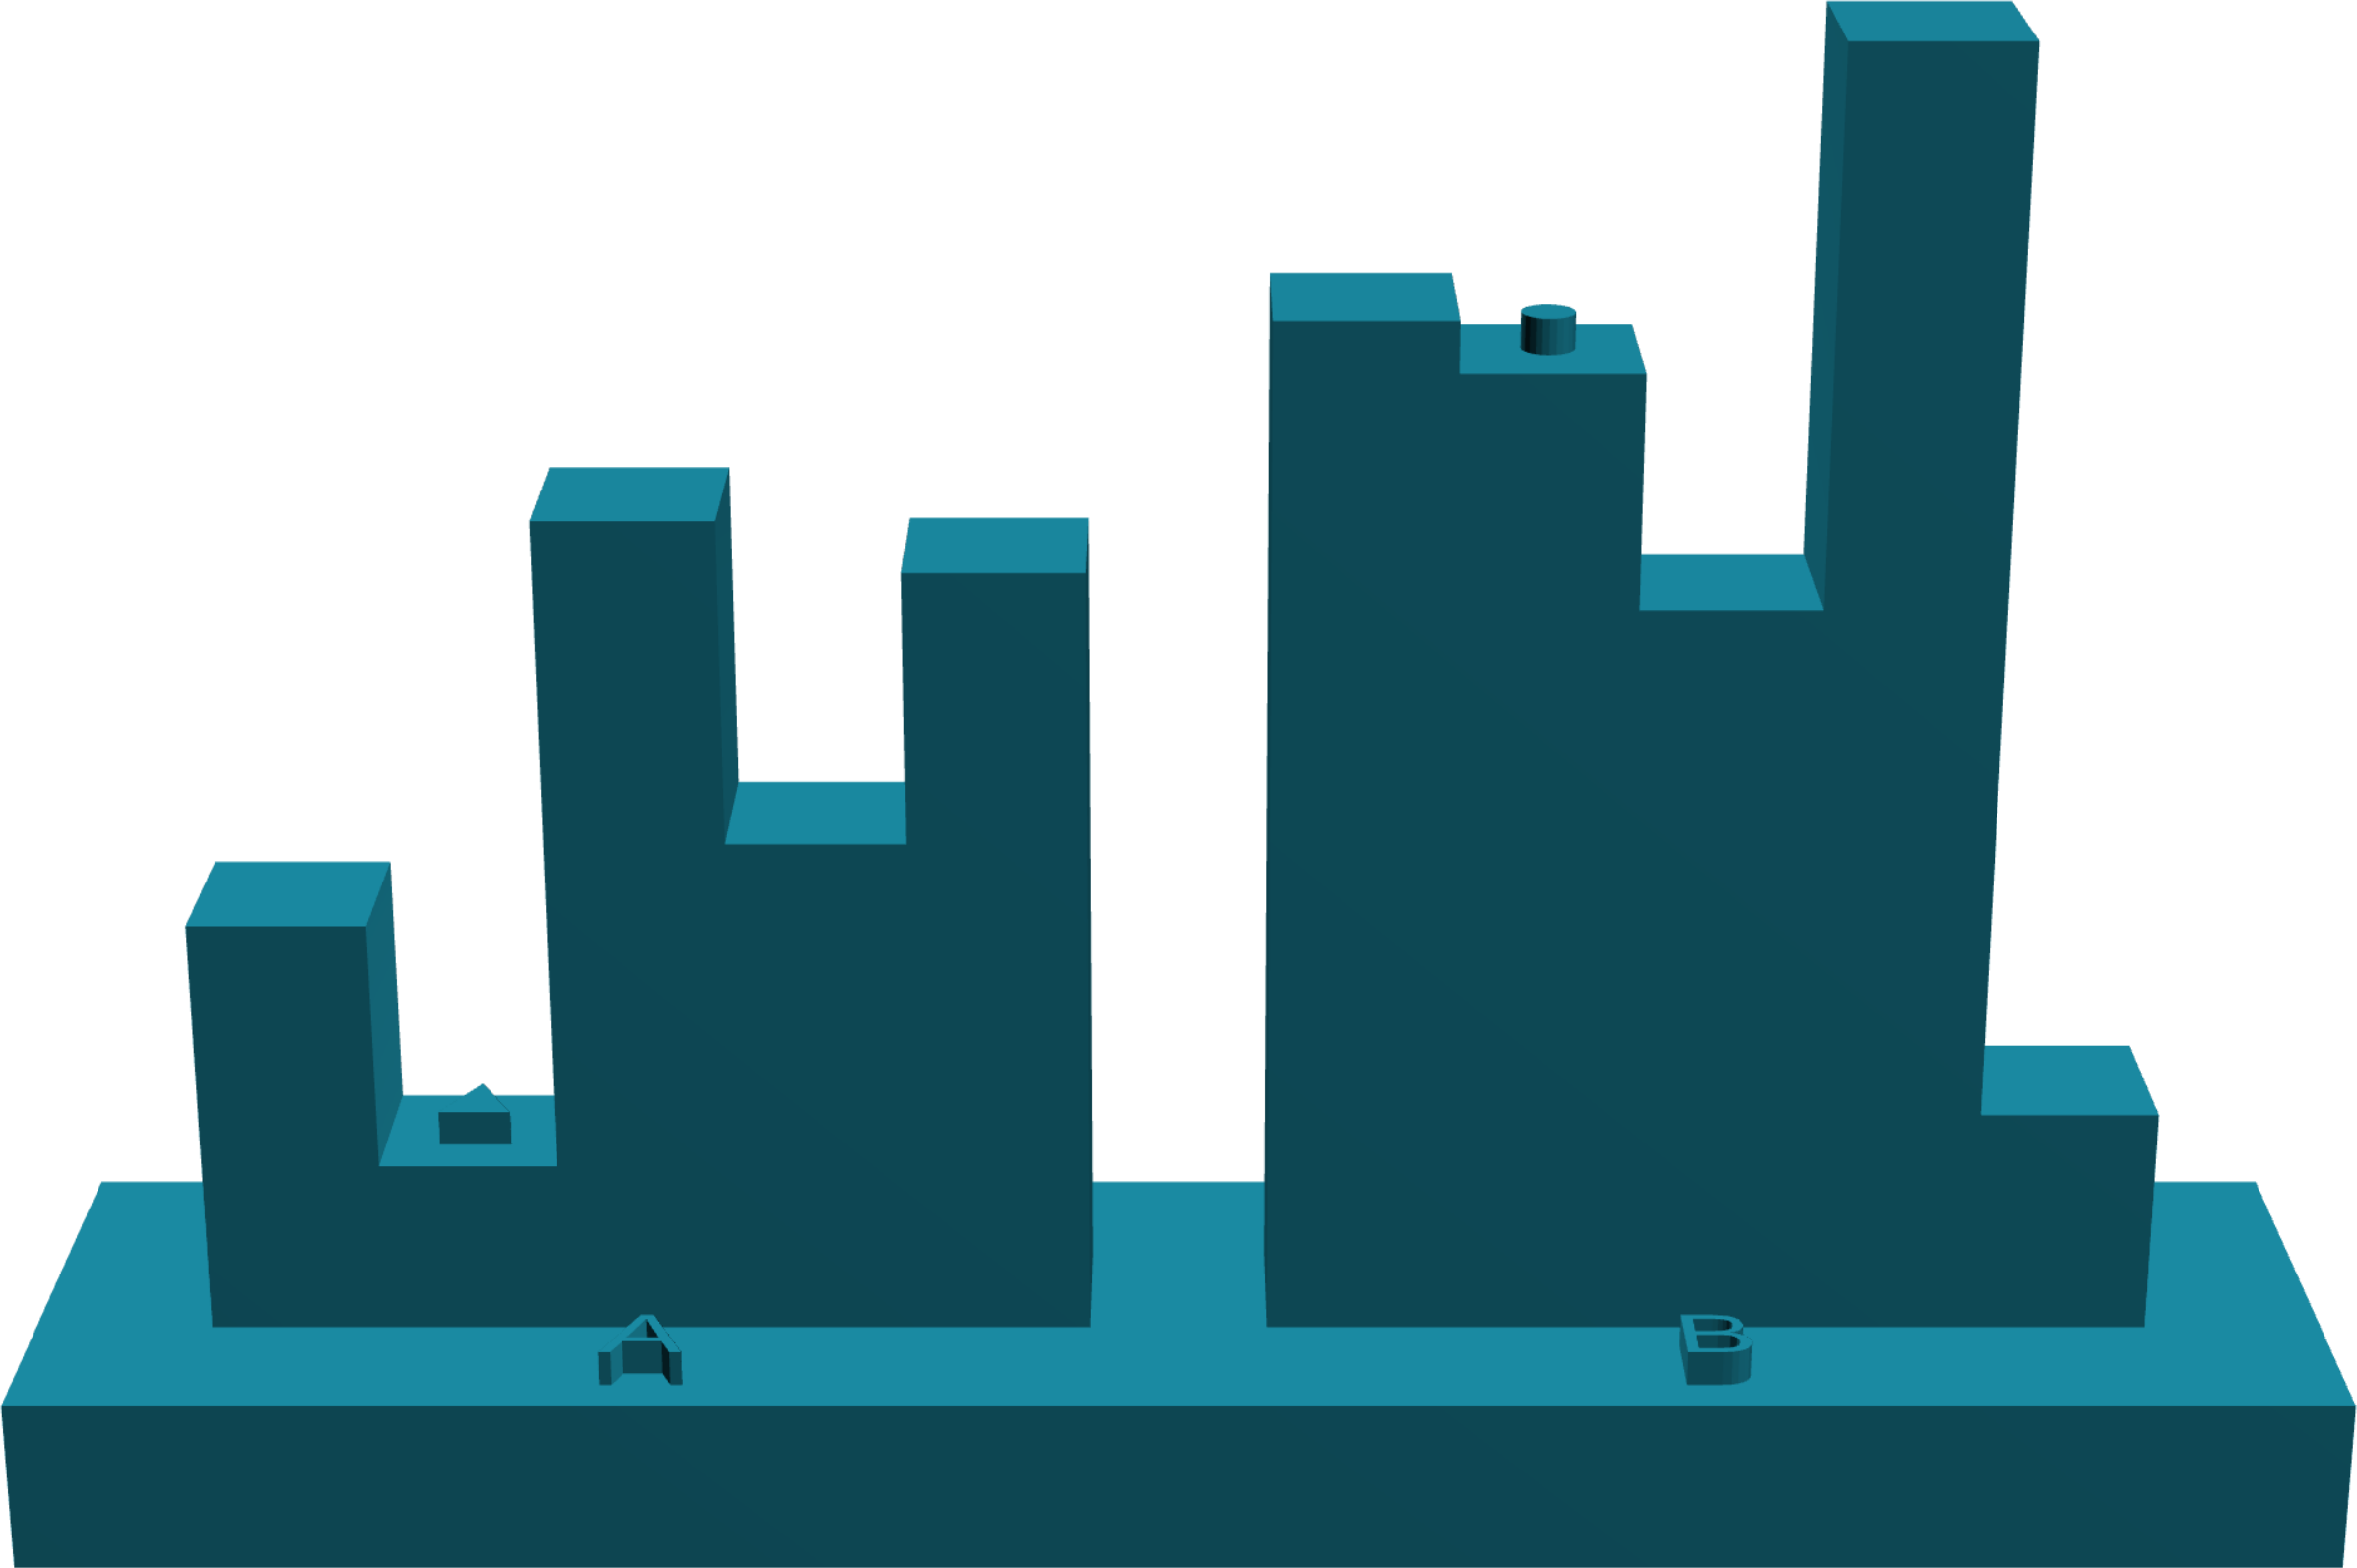
\includegraphics[width=0.3\linewidth]{_images/RenderedChart} 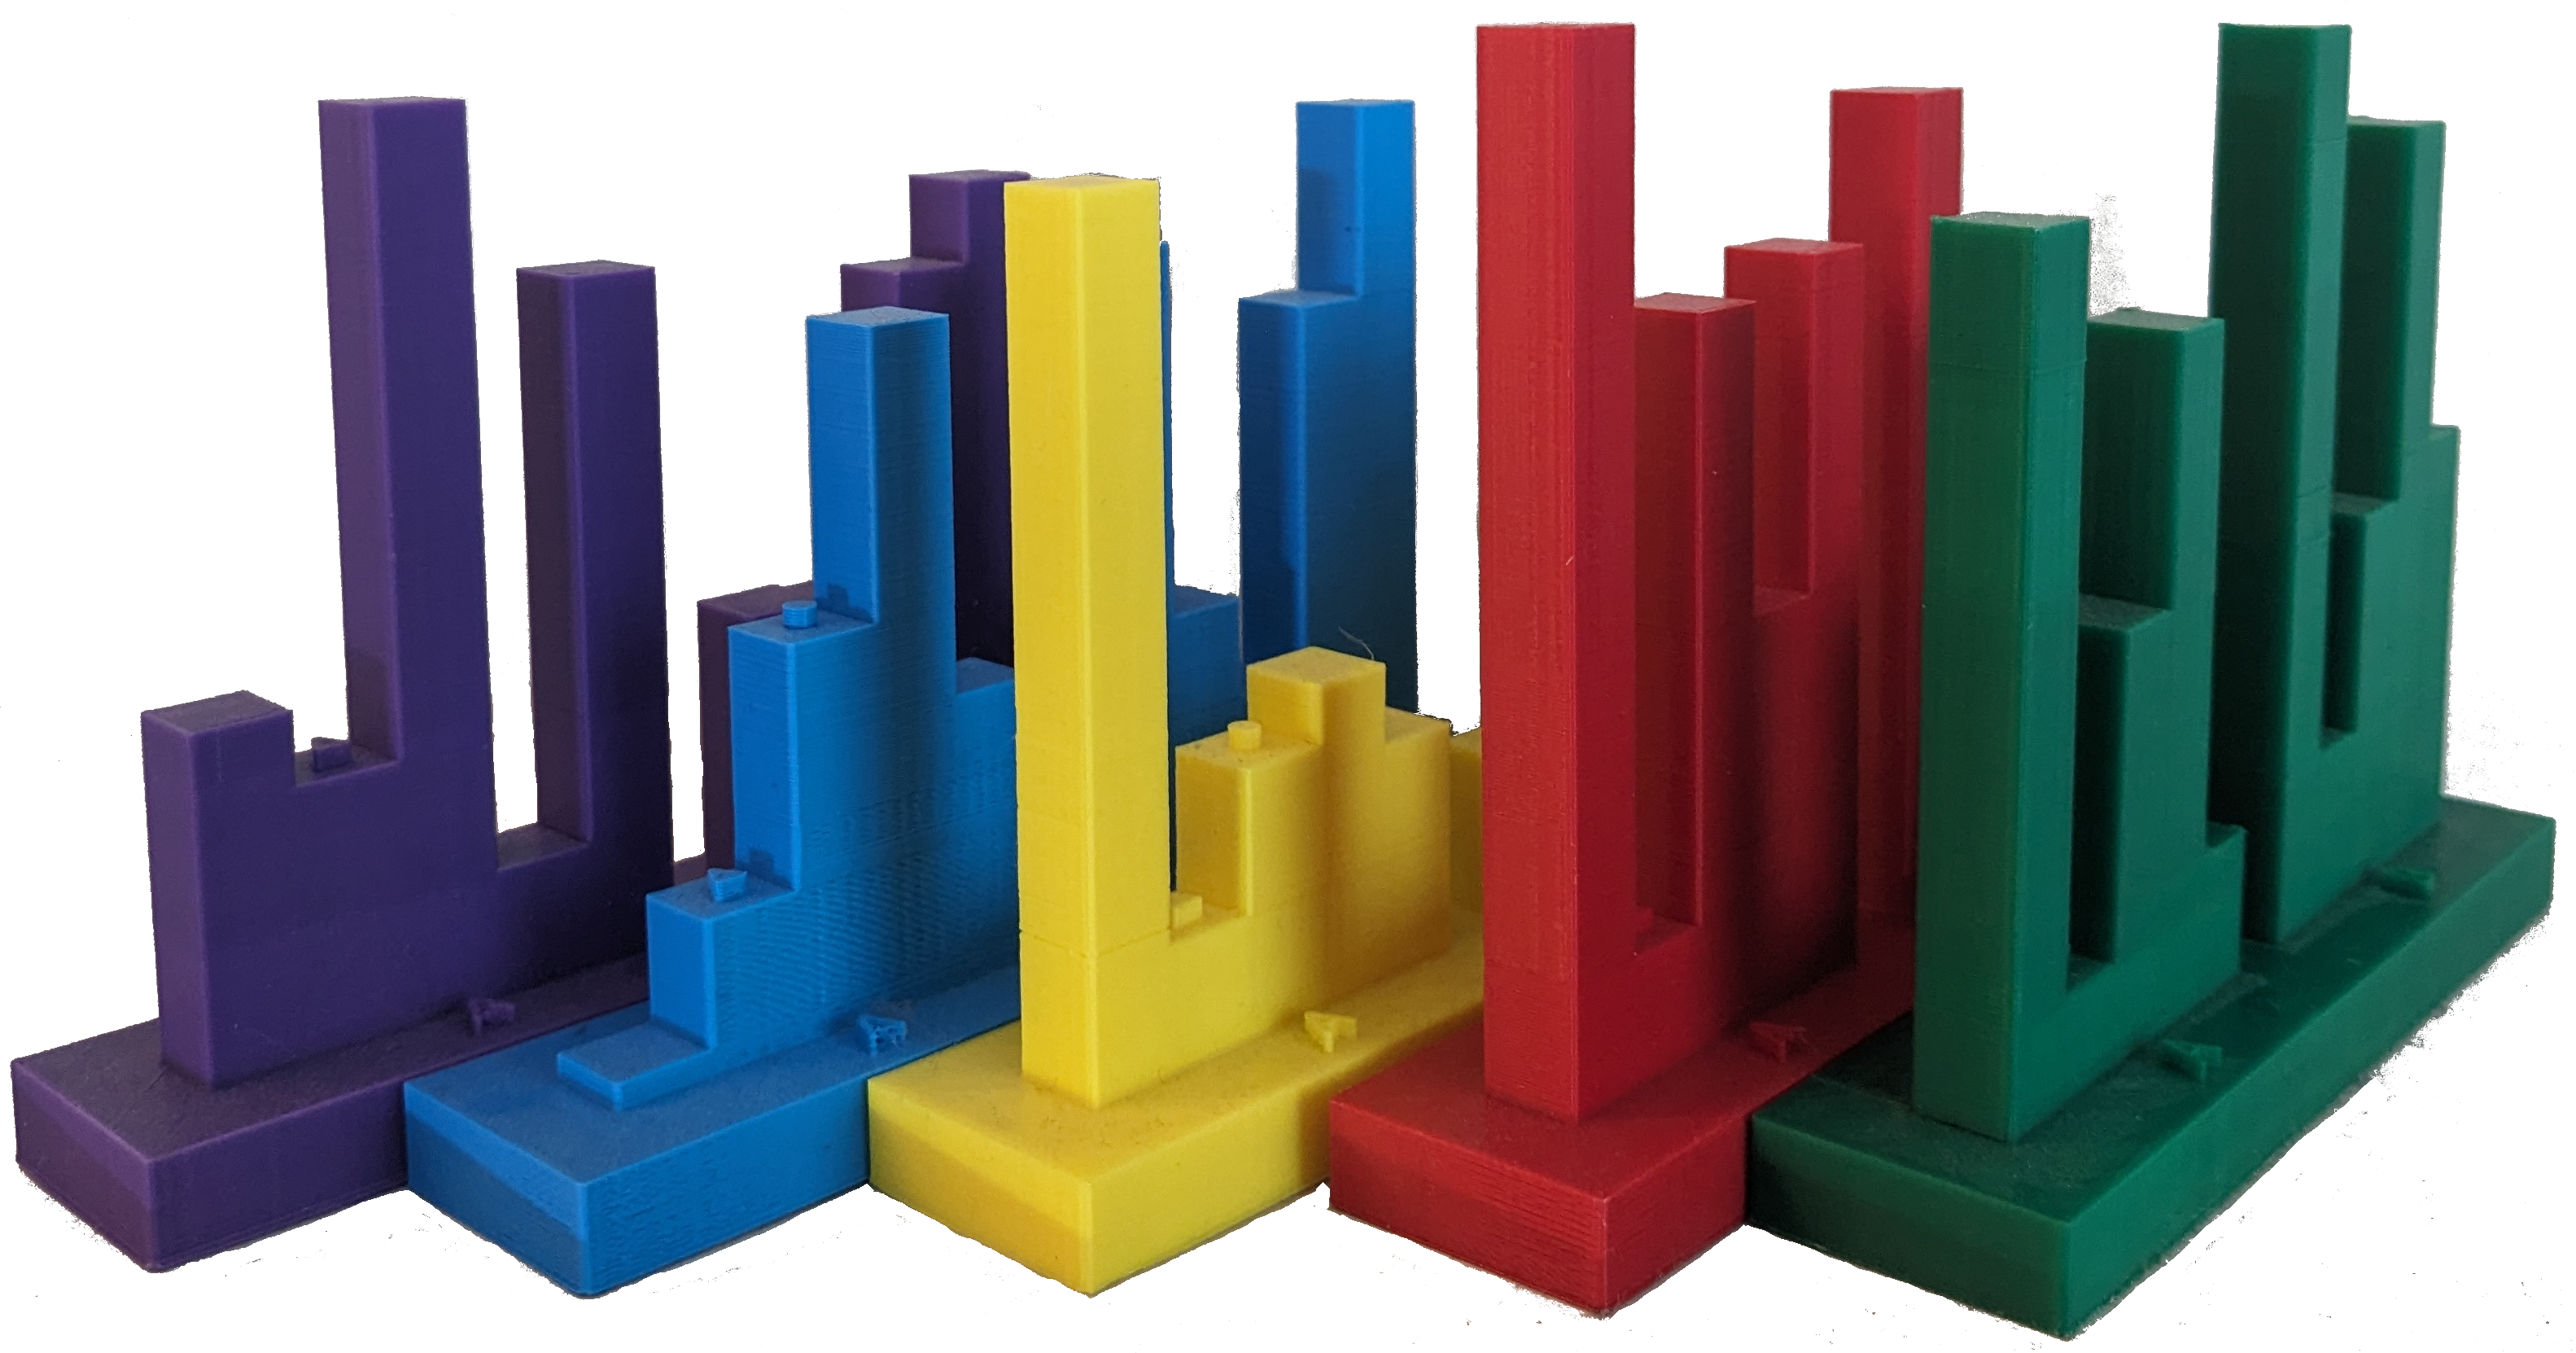
\includegraphics[width=0.35\linewidth]{_images/Kit_of_charts} \caption{Two dimensional, 3D digital rendering, and 3D-printed charts used in this study.}\label{fig:plotTypes}
\end{figure}

The ggplot2 \citep{ggplot2} package was utilized to create the 2D bar charts.
The scale axis was removed, leaving only the bars and a bar grouping identifier.
The bars used for comparisons had the identifying mark at a height of 5 out of 100 for the 2D plots, and the 3D plots had the identifying marks on top of the bars.

The 3D renderings and 3D printed charts were both created using OpenSCAD \citep{kintelOpenSCADDocumentation2023}, which creates STL files from markup describing the object's geometric composition.
Charts were composed of a platform, with raised text labels centered in front of the A and B groups of bars. Bars were created by inserting bar heights into the OpenSCAD template using R, and then raised circle and triangle markers were positioned on top of the bars to be compared to provide a tactile and visual indicator.
In addition, an ID code was engraved into the bottom of the platform to uniquely identify each object; this allowed the researchers to ensure that each kit contained the correct charts throughout the experiment while minimizing the risk of stickers or other identifiers becoming detached from the charts.
As printed, the base of each chart was 13cm x 3cm x 1cm, with the highest bar rising 9.5cm above the chart base.
Raised letters and shapes were 2mm above the base or bar, respectively.
The color of the filament used to print each chart corresponded to the estimation ratio (though this was not obvious to participants), allowing the researchers to quickly determine that a kit of 3D charts contained no ratio duplication.
Colors were randomly assigned to ratios so that participants could not gain information about the ratio from any perceived ordering of the colors.

Digital renderings of the generated STL files were created using RGL \citep{rgl}, which integrates into Shiny \citep{shiny} using the WebGL \citep{mozillafoundationWebGL2D3D2023} extension.
The RGL rendering of the STL file was initially angled to correspond to the perspective of default 3D bar charts present in Microsoft Excel, but in the WebGL interactive environment, participants could rotate the charts as they pleased to create a useful estimate of the bar ratio.
Rendered charts were colored to correspond with the filament color used to print the physical chart for consistency.
The default \texttt{rgl} lighting was replaced with three lights located in fixed positions around the rendered figure.
The lights were positioned so that one was behind the rendered figure, another in front of the figure, and one light below the figure.
This arrangement provided a consistent visual experience and minimized shadows that prevented visual estimation of the bars.

\hypertarget{experiment-design}{%
\subsection{Experiment Design}\label{experiment-design}}

A diagram of the experimental design is provided in \Cref{fig:studyDesign}. The study is set up as a modified randomized incomplete block design, comprised of 3 blocks (presentation mode), 7 bar ratios (5 are selected for each participant). At each combination of ratio and presentation type, the comparison type, adjacent (Type 1) or separated (Type 3), is randomly selected. This process was used to create 21 kits of 5 3D printed charts and 10 virtual charts. There is thus a slight deviation from a completely randomized incomplete block design, in that all possible combinations of ratios, presentation modes, and comparison types are not present in our design. However, this approach provided the best experimental design given the constraints of managing physical stimuli; it took nearly a month of continuous 3D printing to create all of the charts for the kits that we assembled. A dataset containing the kit composition breakdown is available in the github repository for this project.

\begin{figure}
\centering
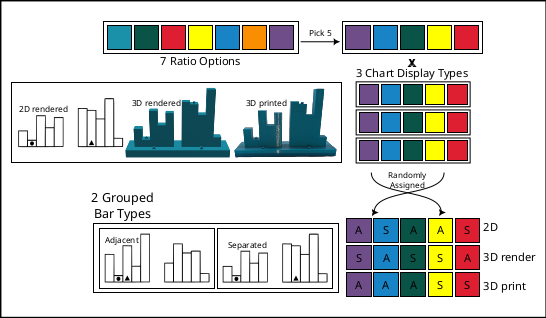
\includegraphics{_images/design.pdf}
\caption{\label{fig:studyDesign}A graphical representation of the study design. Only five of the seven ratios were used in each kit; at least one of the smallest or largest ratios were included along with 4 other charts; each selected ratio was displayed in all 3 mediums. For each medium \(\times\) ratio combination, the comparison type (separated or adjacent) was randomly determined. A total of 21 kits of 3D printed charts were created to include all combinations of the five ratios.}
\end{figure}

\hypertarget{participant-recruitment}{%
\subsection{Participant Recruitment}\label{participant-recruitment}}

One interesting facet of \citet{clevelandGraphical1984} is the participant recruitment methodology: ``For each experiment the subjects fell into two categories: (1) a group of females, mostly housewives, without substantial technical experience; (2) a mixture of males and females with substantial technical training and working in technical jobs.
Most of the subjects in the position-length experiment participated in the position-angle experiment; in all cases repeat subjects judged the position-angle graphs first.''
It seems likely that the authors recruited individuals within their respective departments as well as their wives.
In order to replicate this atypical participant recruitment method in the modern era, members of the UNL Statistics department and their spouses, partners, and roommates were asked to participate in our study.
This replicates the spirit of the recruitment method without the implicit assumptions that graduate students and professors are male, heterosexual, and have unemployed spouses.

A total of 48 participants completed the study; demographics are shown in \Cref{fig:demographics}.

\begin{figure}
\includegraphics[width=1\linewidth]{jds_files/figure-latex/demographics-1} \caption{Demographic characteristics of participants in the study.}\label{fig:demographics}
\end{figure}

While the results of any sample with recruitment methodology like this are not generalizable to the public, running our initial study on a comparable population to that of the initial study serves a purpose: other replications, such as \citet{heerCrowdsourcingGraphicalPerception2010b}, used online samples of paid participants, who likely have less experience using charts and graphics and making numerical estimations than those in a statistics department (and individuals who cohabitate with them). We have every intention of running this experiment in other populations, but the convenience of online sampling is not compatible with physical objects such as our 3D printed charts, so we will have to recruit in-person participants. Thus, an initial study in a population comparable to \citet{clevelandGraphical1984} is a reasonable first step into testing 3D charts.

\hypertarget{data-collection}{%
\subsection{Data Collection}\label{data-collection}}

A Shiny applet was used for data collection, along with the provided kit of 3D printed charts.
Participants provided informed consent through the applet, and then were asked for demographic information (age, gender, education level).
Then, participants were shown a ``practice'' page which allowed them to experiment with the data collection interface and practice estimating the ratio between the bars, as shown in \Cref{fig:practice}. This practice interface did not provide any feedback as to participant correctness, but was merely intended to familiarize the participants with the questions which would be asked as well as the process of estimating the ratio between the two bars.

\begin{figure}
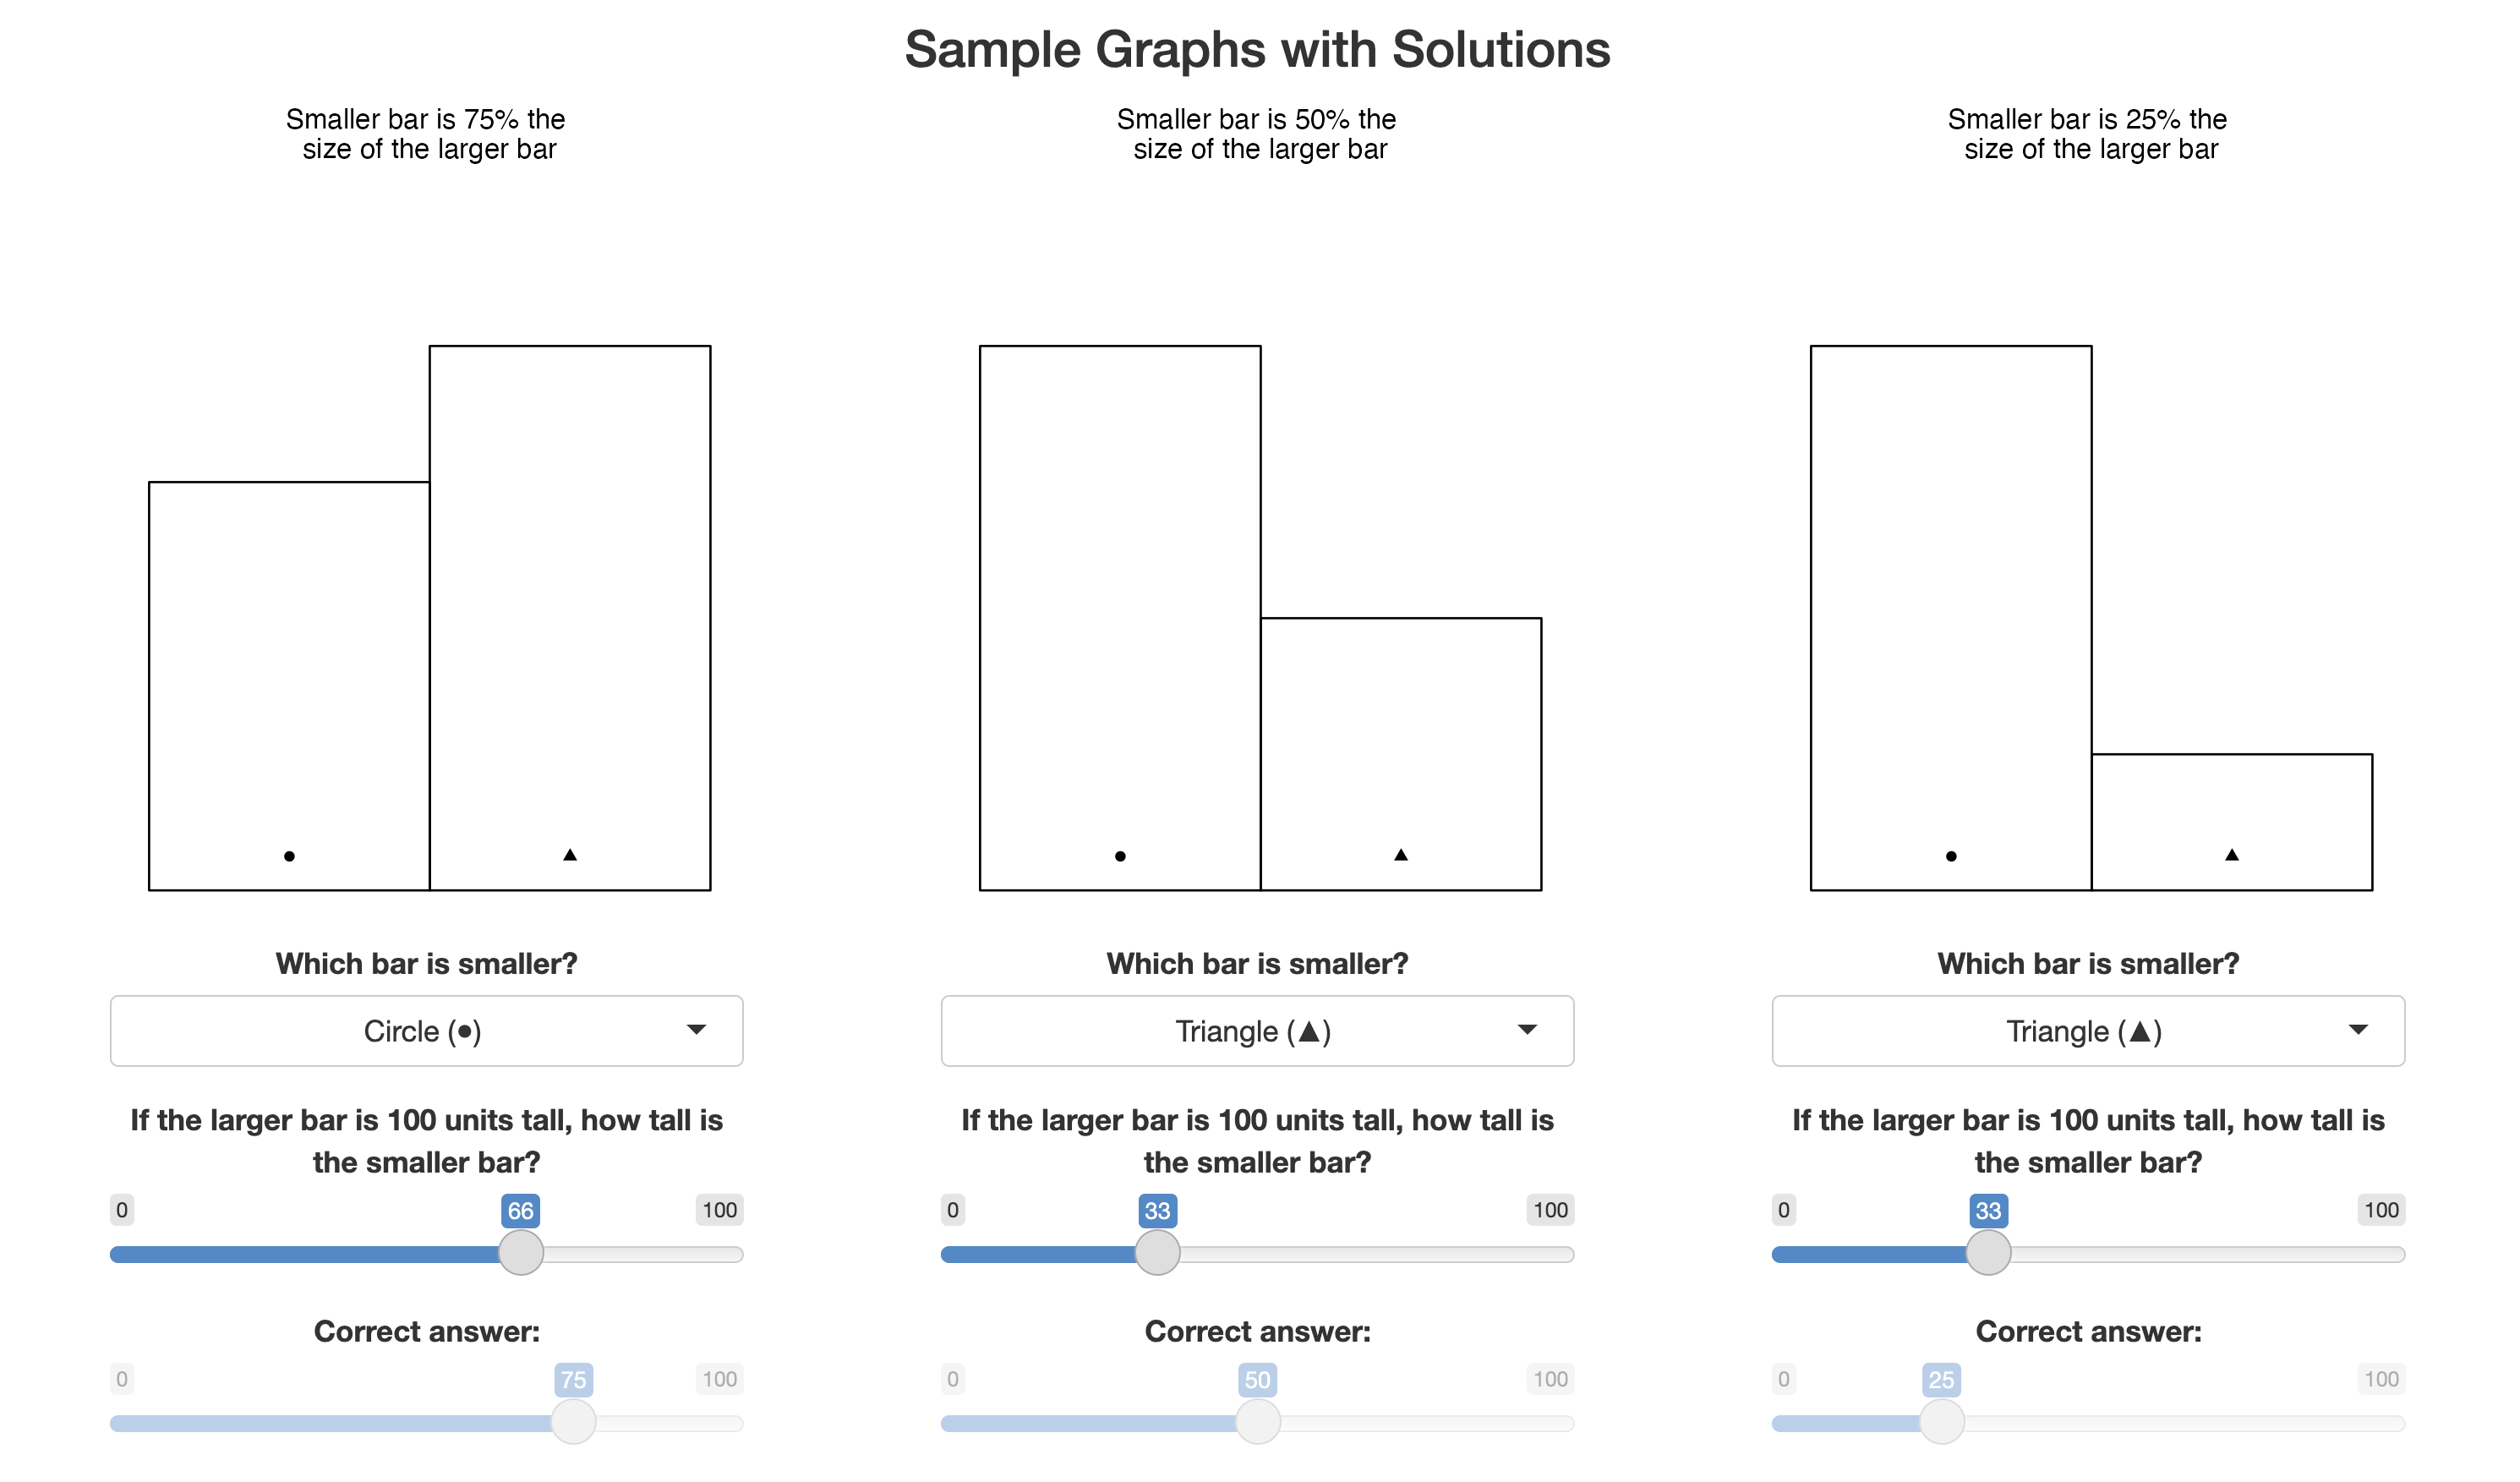
\includegraphics[width=0.8\linewidth]{_images/03-Practice-2} \caption{Screenshot of Shiny application practice screen. Three 2D bar charts with different ratios were provided, along with sliders indicating the correct proportion. Participants could practice with the sliders and preview the questions that would be asked as part of the task.}\label{fig:practice}
\end{figure}

After the practice screen, participants were asked to provide the kit ID. Participants were also instructed that when indicated, they should choose a 3D chart from the kit and select the ID code of the chart (inscribed on the bottom) from the drop-down menu before completing the estimation task.
Participants were also instructed to make quick judgements for each graph and not to measure or estimate ratios using physical objects.

\begin{figure}
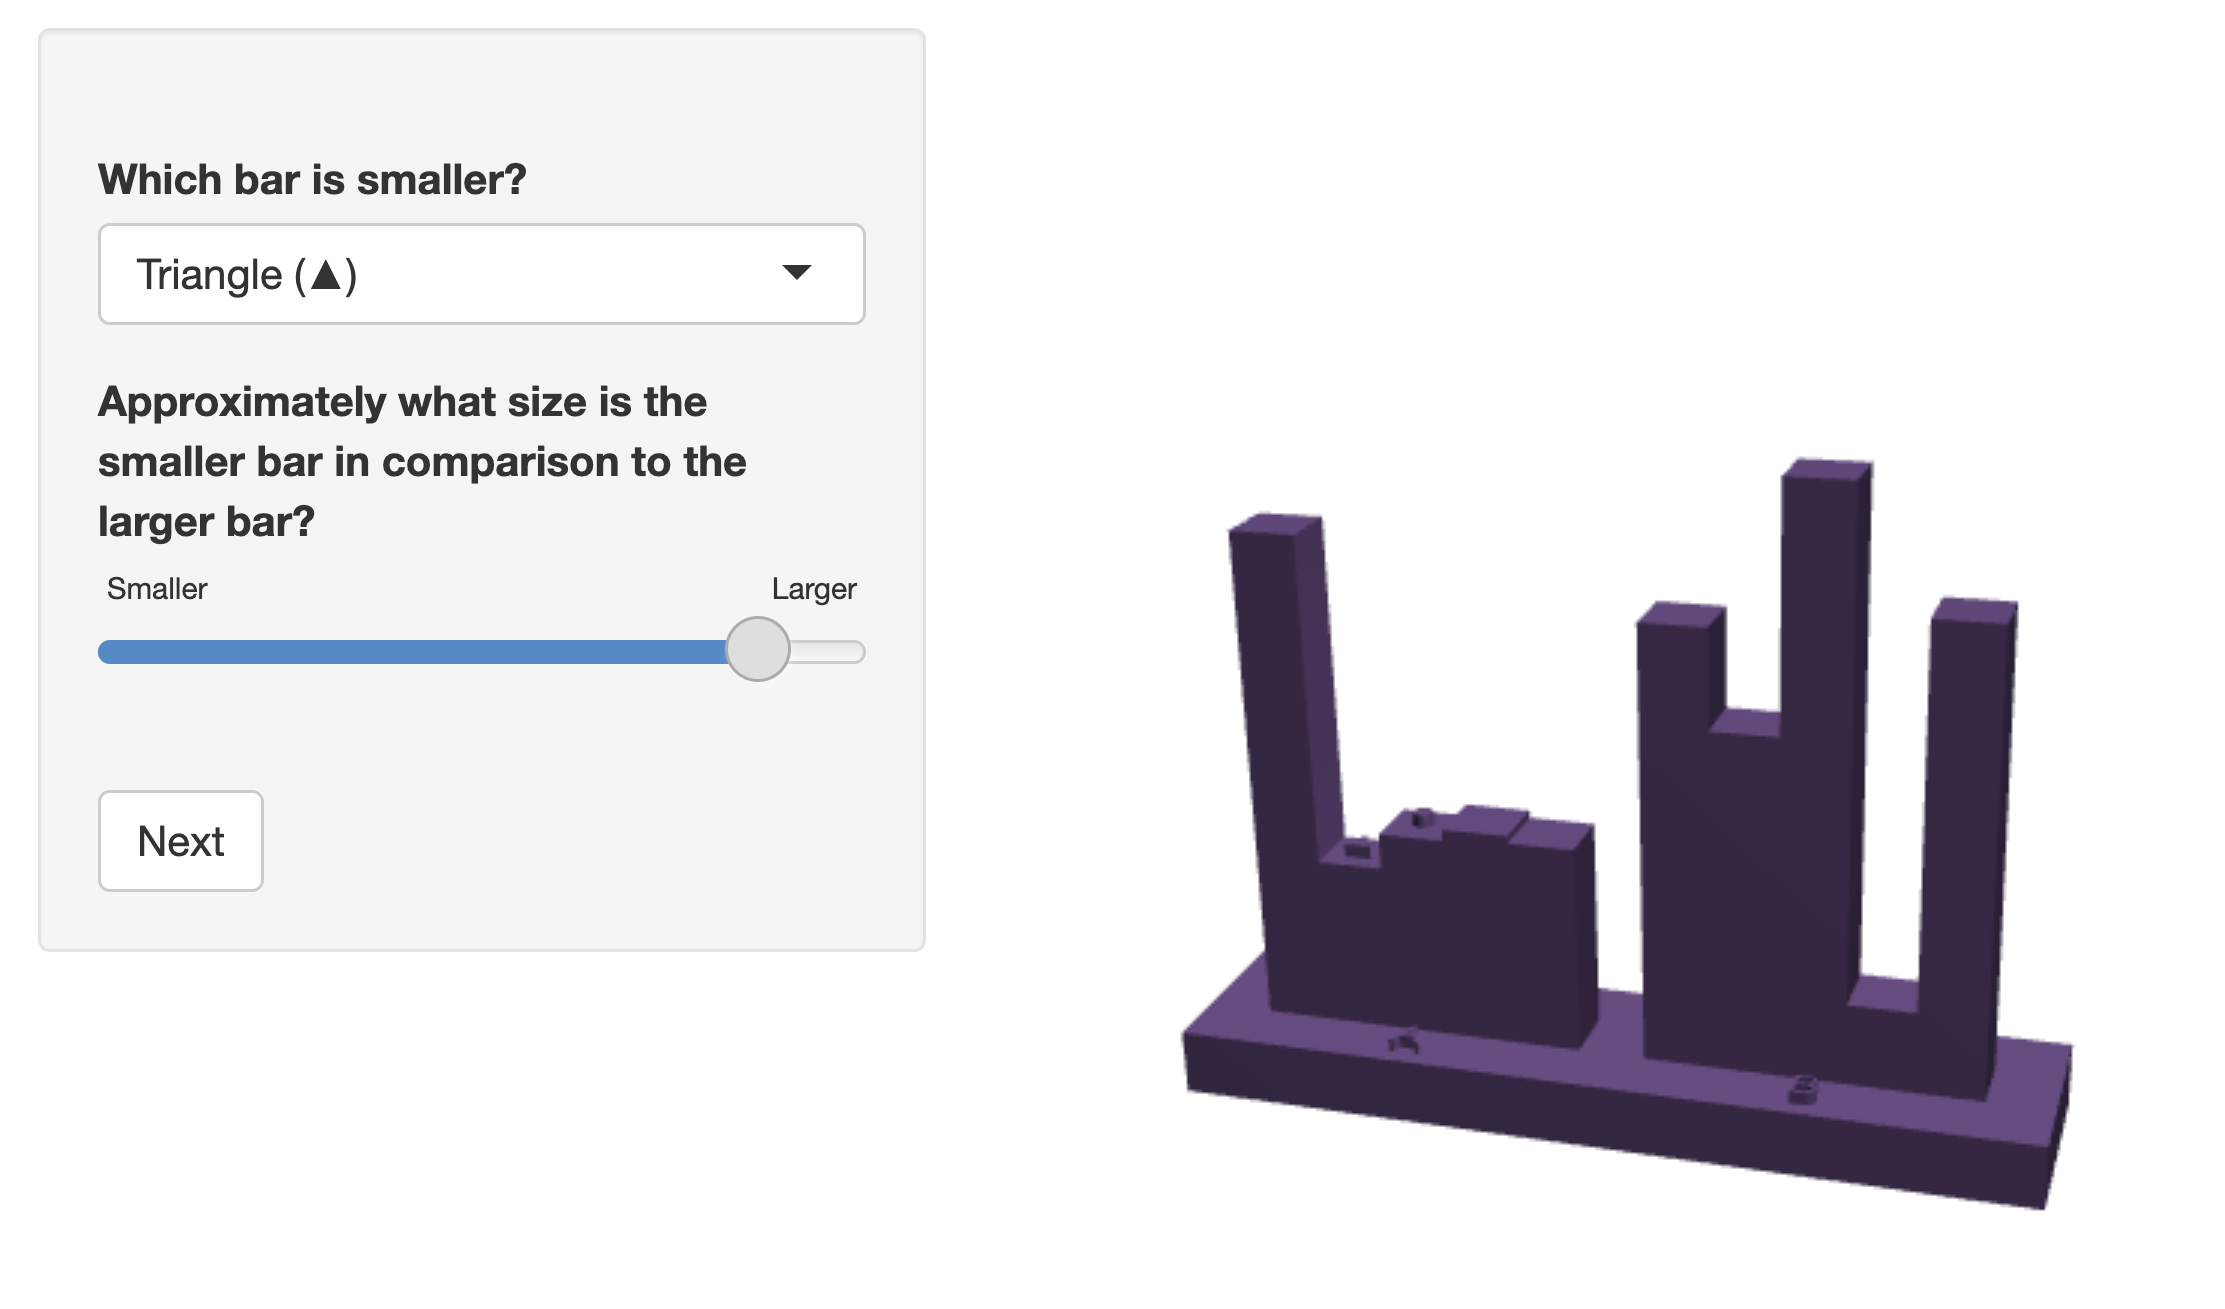
\includegraphics[width=0.8\linewidth]{_images/05-Experiment-05-filled-in} \caption{Screenshot of the applet collecting data for a 3D rendered chart task. Participants were asked to select which bar (circle or triangle) was smaller, and then to estimate the ratio of the smaller bar to the larger bar.}\label{fig:experiment3dRender}
\end{figure}

Each graph (or prompt, in the case of 3D printed charts) in the applet had two corresponding questions for participants to answer: first, participants were to identify the smaller bar by shape, and then, participants were to estimate the ratio of the size of the smaller bar to the size of the larger bar, as shown in \Cref{fig:experiment3dRender}.
It should be noted that we chose to use a slider for entering ratio estimates - in part, this was intended to alleviate rounding effects which occur when participants enter numbers on their own or get numeric feedback from slider entries \citep{ruudUncertaintyCausesRounding2014a, maineriSliderBarsMultiDevice2021}.
Another benefit of this modification is that it should reduce participants' cognitive load, allowing them to focus on the ratio between bars rather than the numerical translation process.
This differs from \citet{clevelandGraphical1984}, but maintains the spirit of the study while using methods which were not available for data entry at the time.

\hypertarget{results}{%
\section{Results}\label{results}}

All responses (\(n = 32\)) that incorrectly identified the smaller bar were removed from the study before analysis; this serves as a basic attention check.

\hypertarget{midmeans-of-log-absolute-errors}{%
\subsection{Midmeans of Log Absolute Errors}\label{midmeans-of-log-absolute-errors}}

\citeauthor{clevelandGraphical1984} used
\[\log_2(|\text{Judged Percent} - \text{True Percent}|+1/8)\]
to measure accuracy of their participant's responses.
In their study, log base 2 seemed appropriate due to ``average relative errors changing by factors less than 10.''
They also added 1/8 to prevent distortions when the errors were close to zero.
\citet{heerCrowdsourcingGraphicalPerception2010b} followed the same analysis method, replicating many (but not all) of the results presented in the original paper.

\Cref{fig:midmeans-log-errors} shows the midmeans of the log absolute errors compared to the true ratio of the bars for each graph type and comparison type.
The results suggest that the log absolute errors increase for greater differences between the smaller and larger bars, but are consistent across the graph types. In addition, there is a tendency

\begin{figure}
\includegraphics[width=0.8\linewidth]{jds_files/figure-latex/midmeans-log-errors-1} \caption{Midmeans and observed values of log absolute errors for the true ratio of bars. Summary lines are computed from raw data using a loess smooth.}\label{fig:midmeans-log-errors}
\end{figure}

This is somewhat different than the results in \citet{clevelandGraphical1984} and \citet{heerCrowdsourcingGraphicalPerception2010b}; in both cases the midmean log absolute errors increased until about 55\% of the true proportional difference and then decreased.
It is possible that this difference is due to the fact that we did not require an explicit numerical estimate of the ratio but instead asked participants to indicate the ratio on a slider (which is essentially a number line).
It is possible that this change explains the lack of a difference between chart modalities we see, but there are other potential explanations as well.
One interesting facet of this data is that there is a consistent reduction in log error when the true proportional difference is near 50\%.
This may be because of implicit anchoring - we can typically bisect a span relatively accurately, which means that it might be expected that when the true proportion is near 50\%, we would both notice that and be able to accurately transfer that information to the slider.
This pattern is more noticable in separated (Type 3) comparisons, which also makes sense - as these comparisons are known to be less accurate, a locally minimal error near 50\% with increased error relative to adjacent (Type 1) comparisons could easily explain the exaggerated trends we see in \Cref{fig:midmeans-log-errors}.

\hypertarget{linear-mixed-effects-model}{%
\subsection{Linear Mixed Effects Model}\label{linear-mixed-effects-model}}

In addition to replicating the (primarily graphical) analysis of participant errors, we also took a more statistical approach and fitted a linear mixed effects model that accounts for participant variation as well as the effect of comparison type, graph type, and ratio. This allows us to test for significant differences (though given the midmean log absolute error plots, we do not expect to find any) as well as to quantify effect sizes for future studies. The formal statistical model is as follows:

\[y_{ijklm}=\mu+S_i + R_j + G_k +T_l + \epsilon_{ijklm}\]

\noindent where

\begin{itemize}
\item
  \(y_{ijklm}=\log_2(|\text{Judged Percent} - \text{True Percent}|+1/8)\)
\item
  \(S_i\sim N(0,\sigma^2_S)\) is the random effect of the \(i^{th}\) subject
\item
  \(R_j\) is the effect of the \(j^{th}\) ratio
\item
  \(G_k\) is the effect of the \(k^{th}\) display type
\item
  \(T_l\) is the effect of the \(l^{th}\) comparison type
\item
  \(\epsilon_{ijklm}\sim N(0,\sigma^2_\epsilon)\) is the random error
\end{itemize}

\begin{table}[tbp]

\begin{center}
\begin{threeparttable}

\caption{\label{tab:unnamed-chunk-2}Analysis of Fixed Effects}

\begin{tabular}{llll}
\toprule
Term & \multicolumn{1}{c}{$\hat{\beta}$} & \multicolumn{1}{c}{95\% CI} & \multicolumn{1}{c}{$t$}\\
\midrule
Intercept & 2.49 & {}[1.94, 3.04] & 8.84\\
Ratio & 0.02 & {}[-0.04, 0.07] & 0.56\\
Plot3dDigital & 0.15 & {}[-0.14, 0.43] & 1.02\\
Plot3dPrint & -0.06 & {}[-0.35, 0.22] & -0.44\\
Type & 0.11 & {}[-0.13, 0.35] & 0.94\\
\bottomrule
\end{tabular}

\end{threeparttable}
\end{center}

\end{table}

No differences were detected for the true ratio of bars (\(t = 0.5590574\)), whether the bars were adjacent or separated (\(t = 0.9381629\)), or for the plot nested within the true ratio (\(F(2, 441) = 1.1110313\)).
While \citeauthor{heerCrowdsourcingGraphicalPerception2010b} provided a zip file containing data and code for their paper, the link is no longer active, so it is not possible to fit a similar model to their data for comparison purposes.

\hypertarget{interactivity-with-3d-rendered-charts}{%
\subsection{Interactivity with 3D Rendered Charts}\label{interactivity-with-3d-rendered-charts}}

When 3D rendered plots were shown, we recorded the number of user interactions (clicks, rotations) with the WebGL plot. \Cref{fig:clicks} shows the distribution of number of clicks over all 3D rendered trials in the experiment, as well as the number of clicks relative to the accuracy measure \(\log_2(|\text{Judged Percent} - \text{True Percent}|+1/8)\). It does not appear that participants who interacted with the WebGL rendering were more accurate than their peers who did not.

\begin{figure}
\includegraphics[width=.45\textwidth]{jds_files/figure-latex/clicks-1} \includegraphics[width=.45\textwidth]{jds_files/figure-latex/clicks-2} \caption{Participant clicks on the WebGL interface (left) in order to interact with the plot. Most participants did not interact with the WebGL interface, perhaps because they did not realize that interacting was an option, but some participants utilized the interactivity heavily. (Right) Participant interactivity was not associated with increased accuracy.}\label{fig:clicks}
\end{figure}

\hypertarget{discussion-and-future-work}{%
\section{Discussion and Future Work}\label{discussion-and-future-work}}

Previous work in 3D graphics would suggest that the errors for the 3D graphs would be larger than the errors for the 2D graphs.
While we did not find any significant results indicating that 3D graphs are read less accurately, there are two possibilities that might account for this discrepancy.

The first potential explanation is that this study is underpowered - the effect size is small, and our 48 participants were insufficient; the original study included 51 participants, which is slightly larger. However, we should note that the analysis methods used in \citet{heerCrowdsourcingGraphicalPerception2010b} and \citet{clevelandGraphical1984} do not provide numerical tests of statistical significance, instead defaulting to graphical displays which include confidence intervals.

The second possibility is more interesting: we examined 3D charts using rendered 3D graphs and 3D printed charts; both of these options allow for participants to interact with the chart, rotating it, and generally perceiving it as one might perceive any other 3D, real, object.
This is a far cry from the 3D perspective charts in the original study, which have a fixed angle and perspective and are thus not equivalent to our 3D charts.
Future studies should include an additional fixed 3D perspective bar chart, which will at least enable us to examine whether modern 3D rendering environments allow for more accurate conclusions than fixed 3D perspectives. Future iterations of this study will include ``traditional'' 3D graphs created by Microsoft Excel (that is, graphs with a fixed 3D perspective rendered in 2D). This option will allow us to examine fixed perspective 3D plots compared to 3D renderings and 2D plots; it will also enable online data collection in addition to the in-person data collection used in this experiment.

Another interesting aspect of our study is that the method used to record participant estimates is different from the method used in the original study as well as Heer \& Bostock's replication study.
A method similar to our slider input, marking position on a line, was used in \citet{spenceVisualPsychophysicsSimple1990}, but Spence asked participants to estimate \(A/(A+B)\), where we asked participants to estimate \(A/B\); thus, our results are still not directly comparable to previous studies.
We expect that the specific ratio estimated would also have an effect on observed participant errors.

The slider method for input of ratio estimates should be easier for participants, as it does not require explicit transformation to the numerical domain.
What is clear is that it would be beneficial to assess the impact of the measurement method on participant errors directly, so that the results of these different studies might be explained and interpreted with regard both to the stimuli used and the measurement method employed in the experiment.
Future iterations of this experiment will likely address this estimation difference; such modifications in experimental design are relatively straightforward in Shiny and will provide useful insight into the design of future experiments evaluating the perception of statistical graphics.

\hypertarget{supplemental-material}{%
\subsection{Supplemental Material}\label{supplemental-material}}

Stimuli, code, and data for this experiment are provided at \url{https://github.com/TWiedRW/2023-JDS-3dcharts}.

\bibliography{JDS2023.bib}
\bibliographystyle{jds}


\end{document}
